\documentclass{standalone}
\author{Quinten Bruynseraede}
\usepackage{tikz}
\usetikzlibrary{shapes}
\title{Tikz grafen}
\begin{document}\pagestyle{empty}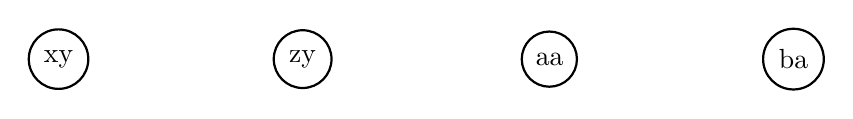
\begin{tikzpicture}\node[shape=circle,draw=black,align=center,line width=0.8pt] (0) at (1.5666666666666667,10.366666666666667) {xy};
\node[shape=circle,draw=black,align=center,line width=0.8pt] (1) at (4.666666666666667,10.366666666666667) {zy};
\node[shape=circle,draw=black,align=center,line width=0.8pt] (2) at (7.8,10.366666666666667) {aa};
\node[shape=circle,draw=black,align=center,line width=0.8pt] (3) at (10.9,10.366666666666667) {ba};

\end{tikzpicture}
\end{document}